\documentclass[]{report}


% Title Page
\title{}
\author{}

\usepackage{bera}% optional: just to have a nice mono-spaced font
\usepackage{listings}
\usepackage{xcolor}
\usepackage{float}
\usepackage{graphicx}
\colorlet{punct}{red!60!black}
\definecolor{background}{HTML}{EEEEEE}
\definecolor{delim}{RGB}{20,105,176}
\colorlet{numb}{magenta!60!black}
\usepackage{xcolor}
\usepackage{amsmath,amsfonts,amssymb}
\newcommand{\source}[1]{\caption*{Source: {#1}} }
\usepackage[hyphens]{url}
\lstdefinelanguage{json}{
	basicstyle=\normalfont\ttfamily,
	numbers=left,
	numberstyle=\scriptsize,
	stepnumber=1,
	numbersep=8pt,
	showstringspaces=false,
	breaklines=true,
	frame=lines,
	backgroundcolor=\color{background},
	literate=
	*{0}{{{\color{numb}0}}}{1}
	{1}{{{\color{numb}1}}}{1}
	{2}{{{\color{numb}2}}}{1}
	{3}{{{\color{numb}3}}}{1}
	{4}{{{\color{numb}4}}}{1}
	{5}{{{\color{numb}5}}}{1}
	{6}{{{\color{numb}6}}}{1}
	{7}{{{\color{numb}7}}}{1}
	{8}{{{\color{numb}8}}}{1}
	{9}{{{\color{numb}9}}}{1}
	{:}{{{\color{punct}{:}}}}{1}
	{,}{{{\color{punct}{,}}}}{1}
	{\{}{{{\color{delim}{\{}}}}{1}
	{\}}{{{\color{delim}{\}}}}}{1}
	{[}{{{\color{delim}{[}}}}{1}
	{]}{{{\color{delim}{]}}}}{1},
}
\begin{document}
\maketitle


\section{Les étapes principales}

\section{Résultat I}
\subsection{Inputs}
\begin{verbatim}
{
	"comment": " June 2016", 
	"af": "", 
	"minASNEntropy": 0.5, 
	"alpha": 0.01, 
	"end": {
		"$date": 1477024630000
	}, 
	"binMult": 3, 
	"timeWindow": 3600,
	"minSeen": 3, 
	"start": {
		"$date": 1477010230000
		
	}, 
	"minASN": 3, 
	"nbProcesses": 24, 
	"experimentDate": {
		"$date": 1456747743895
	}, 
	"confInterval": 0.05,
	"prefixes": "",
	"msm" : 5004,
	"table": "traceroutes_api"
	
}


\end{verbatim}
\subsection{Outputs}

\section{Résultat II}
\subsection{Inputs}

\begin{verbatim}
 expParam = {
					"timeWindow": 60*60, # in seconds 
					"start": datetime(2017, 5, 1, 0, 0, tzinfo=timezone("UTC")),
					"end":   datetime(2017, 5, 1, 4, 0, tzinfo=timezone("UTC")),
					"alpha": 0.01, 
					"confInterval": 0.05,
					"minASN": 3,
					"minASNEntropy": 0.5,
					"minSeen": 3,
					"experimentDate": datetime.now(),
					"af": "",
					"comment": "Study case for Emile (8.8.8.8) Nov. 2016",
					"prefixes": None
					}
\end{verbatim}

\subsection{Outputs}

\begin{verbatim}

> db.rttChanges.findOne()
{
	"_id" : ObjectId("5b6d5dc2c3bb4e36f2f298a7"),
	"currLow" : 0.1739999999999995,
	"nbProbes" : 59,
	"diff" : 0.14300000000000068,
	"trimDist" : false,
	"nbSamples" : 59,
	"msmId" : {
		"5001" : [
		13755,
		13519,
		15653,
		13758,
		25087
		]
	},
	"nbSeen" : 3,
	"ref" : -2.762999999999998,
	"deviation" : 1.1127415891195425,
	"timeBin" : ISODate("2016-10-04T00:00:00Z"),
	"refLow" : -2.8740000000000023,
	"ipPair" : [
	"46.17.232.13",
	"46.17.234.15"
	],
	"asnEntropy" : 0.9209727312690482,
	"samplePerASN" : [
	30969,
	30844,
	37183
	],
	"devBound" : 0.05118110236220502,
	"refHigh" : 0.030999999999998806,
	"diffMed" : 3.108999999999998,
	"nbASN" : 3,
	"median" : 0.3460000000000001,
	"currHigh" : 0.7830000000000013,
	"expId" : ObjectId("5b6d5261c3bb4e36f2f298a6")
}
\end{verbatim}

\section{Caractérisation d'un lien}
\subsection{Echantillon de traceroutes}
\begin{lstlisting}[language=json,firstnumber=1]
{
	"lts":113,
	"size":40,
	"from":"196.216.164.50",
	"dst_name":"192.5.5.241",
	"fw":4780,
	"proto":"UDP",
	"af":4,
	"msm_name":"Traceroute",
	"stored_timestamp":1514768501,
	"prb_id":14465,
	"result":[
	{
		"result":[
		{
			"rtt":2.201,
			"ttl":255,
			"from":"196.216.164.1",
			"size":28
		},
		{
			"rtt":1.917,
			"ttl":255,
			"from":"196.216.164.1",
			"size":28
		},
		{
			"rtt":1.923,
			"ttl":255,
			"from":"196.216.164.1",
			"size":28
		}
		],
		"hop":1
	},
	{
		"result":[
		{
			"rtt":0.579,
			"ttl":254,
			"from":"196.12.10.246",
			"size":28
		},
		{
			"rtt":0.531,
			"ttl":254,
			"from":"196.12.10.246",
			"size":28
		},
		{
			"rtt":0.544,
			"ttl":254,
			"from":"196.12.10.246",
			"size":28
		}
		],
		"hop":2
	},
	{
		"result":[
		{
			"rtt":1.078,
			"ttl":253,
			"from":"160.242.100.88",
			"size":28
		},
		{
			"rtt":0.762,
			"ttl":253,
			"from":"160.242.100.88",
			"size":28
		},
		{
			"rtt":0.698,
			"ttl":253,
			"from":"160.242.100.88",
			"size":28
		}
		],
		"hop":3
	},
	{
		"result":[
		{
			"rtt":64.236,
			"ttl":252,
			"from":"196.216.48.144",
			"size":28
		},
		{
			"rtt":64.213,
			"ttl":252,
			"from":"196.216.48.144",
			"size":28
		},
		{
			"rtt":64.24,
			"ttl":252,
			"from":"196.216.48.144",
			"size":28
		}
		],
		"hop":4
	},
	{
		"result":[
		{
			"x":"*"
		},
		{
			"x":"*"
		},
		{
			"x":"*"
		}
		],
		"hop":5
	},
	{
		"result":[
		{
			"rtt":182.876,
			"ttl":248,
			"from":"196.49.6.10",
			"size":28
		},
		{
			"rtt":182.268,
			"ttl":248,
			"from":"196.49.6.10",
			"size":28
		},
		{
			"rtt":182.288,
			"ttl":248,
			"from":"196.49.6.10",
			"size":28
		}
		],
		"hop":6
	},
	{
		"result":[
		{
			"rtt":185.761,
			"ttl":56,
			"from":"192.5.5.241",
			"size":28
		},
		{
			"rtt":185.728,
			"ttl":56,
			"from":"192.5.5.241",
			"size":28
		},
		{
			"rtt":185.798,
			"ttl":56,
			"from":"192.5.5.241",
			"size":28
		}
		],
		"hop":7
	}
	],
	"timestamp":1514768400,
	"src_addr":"196.216.164.50",
	"paris_id":1,
	"endtime":1514768404,
	"type":"traceroute",
	"dst_addr":"192.5.5.241",
	"msm_id":5004
}

\end{lstlisting}

\begin{lstlisting}[language=json,firstnumber=1]
{
	(u'160.242.100.88', u'196.216.48.144'): {
		'rtt': [63.474000000000004], 
		'probe': [u'196.216.164.50'], 
		'msmId':  {5004: set([14465])}}, 
	
	(u'196.49.6.10', u'192.5.5.241'): {
		'rtt': [3.4729999999999848], 
		'probe': [u'196.216.164.50'], 
		'msmId': {5004: set([14465])}}, 
	
	(u'196.216.164.1', u'196.12.10.246'): {
		'rtt': [-1.379], 
		'probe': [u'196.216.164.50'], 
		'msmId': {5004: set([14465])}}, 
	
	(u'196.12.10.246', u'160.242.100.88'): {
		'rtt': [0.21799999999999997], 
		'probe': [u'196.216.164.50'], 
		'msmId':  {5004: set([14465])}}
}
\end{lstlisting}

\paragraph{Traceroute de base}

\paragraph{Differential RTT computation}
Soit un traceroute depuis la sonde $P$ vers une destination $D$. Soient $X$ et $Y$ les deux routeurs impliqués dans le trafic entre $P$ et $D$.

\begin{figure}[H]
\centering
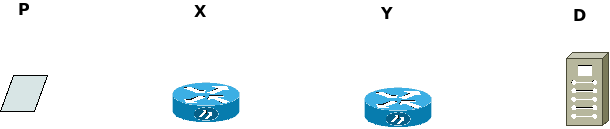
\includegraphics[width=0.7\linewidth]{dia/traceroute}
\caption{}
\label{fig:traceroute}
\end{figure}

La sonde $P$ lance $3$ signaux vers chaque routeur. Le nombre $3$ dépend de l'implémentation du traceroute.  
On note de $1$ à $9$ à RTTs différentiel entre $P$ et $X$. Soit $RTT_{PX}$ le RTT entre la sonde P et le routeur $X$. Ainsi, on note $RTT_{PX1}$, $RTT_{PX2}$ et $RTT_{PX3}$ les RTTs entre $P$ et $X$. Le RTT différentiel du lien $XY$ peut être calculé via $9$ valeurs : 
\begin{itemize}
	\item ($RTT_{PY1}$ - $RTT_{PX1}$)
	\item ($RTT_{PY1}$ - $RTT_{PX2}$)
	\item ($RTT_{PY1}$ - $RTT_{PX3}$)
	\item ($RTT_{PY2}$ - $RTT_{PX1}$)
	\item ($RTT_{PY2}$ - $RTT_{PX2}$)
	\item ($RTT_{PY2}$ - $RTT_{PX3}$)	
	\item ($RTT_{PY3}$ - $RTT_{PX1}$)
	\item ($RTT_{PY3}$ - $RTT_{PX2}$)
	\item ($RTT_{PY3}$ - $RTT_{PX3}$)
\end{itemize}

\begin{verbatim}
Our preliminary experiments suggest that the frequent outlying
values found in RTT measurements greatly affect the computed
mean values; thus an impractical number of samples is required for
the CLT to hold. To address this we replace the arithmetic mean
by the median. This variant of the CLT is much more robust to
outlying values and requires less samples to converge to the normal
distribution 
\end{verbatim}
On va calculer la mediane des RTT différentiels, ensuite, on va calculer l'intervalle de confiance.

\paragraph{Note}
Afin de calculer l'incertitude associée à un ensemble de résultats, il faut répéter les mesures. Chaque mesure sur un échantillon peut donner des résultats différents. Ainsi, en se basant sur la déviation sur les résultats, il est possible de calculer l'incertitude de la "moyenne" calculée de ces résultats. Cette incertitude permet de donner une indication sur les données. Par exemple, est ce que la moyenne calculée $N$ représente la valeur réelle avec une incertitude de +- $m$.

\paragraph{Calcul de l'intervalle de confiance}
les intervalles de confiance sont formulés par un calcul binomial avec distribution free. Ce calcul  est approché par le score de Wilson.


\begin{equation}
f(x)=\begin{cases}
\frac{\Delta^{(l)} - \overline{\Delta}^{(u)}}{\overline{\Delta}^{(u)} - \overline{\Delta}^{(m)}}    , & \text{if $\overline{\Delta}^{(u)}<\Delta^{(l)}$}.\\

\frac{\overline{\Delta}^{(l)} - \Delta^{(u)}}{\overline{\Delta}^{(u)} - \overline{\Delta}^{(m)}}, & \text{if $\overline{\Delta}^{(m)}<\Delta^{(l)}$}.\\
0, & \text{otherwise}.
\end{cases}
\end{equation}
\paragraph{Score de Wilson}
\begin{itemize}
	\item Wilson intervall is for 2 variables only.
	\item  Useful wherever you want to make a confident estimate about the actions or preferences of a general population, given a sample of data (e.g. assigning scores for ranking comments by upvotes, products by popularity.
	\item Le score de Wilson a été choisi pour sa performance dans le cas d
	\item Le score de Wilson fournit deux valeurs dans $ [0, 1]$. 
	\item Chaque valeur de médiane a son intervalle de confiance. On compare le chavauchement entre l'intervalle de confiance de la médiane référence avec l'intervalle de confiance de la valeur de médiane en cours. Afin d'évaluer si la différence entre ces deux intervalles est significative statistiquement. En particulier une différence de $1$ $ms$ est non significative.
\end{itemize}

\begin{figure}[H]
\centering
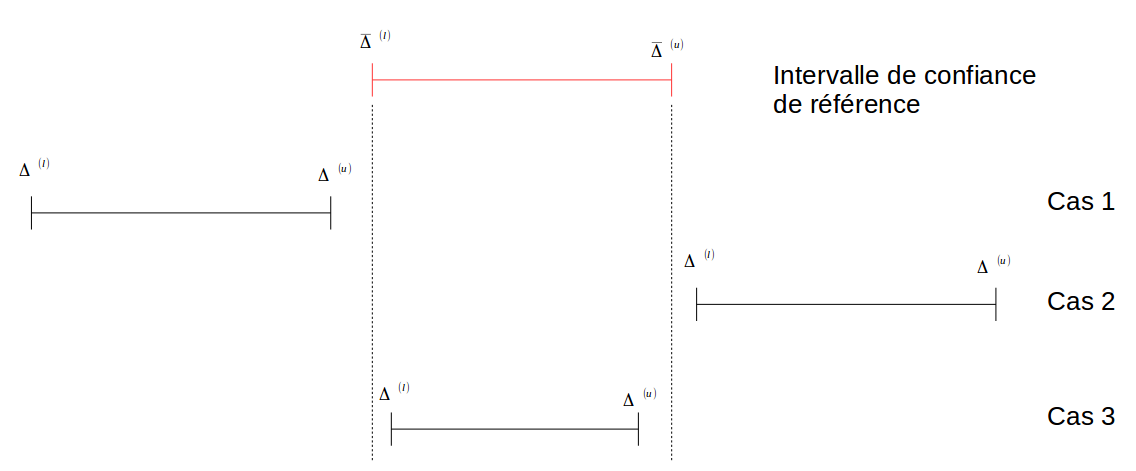
\includegraphics[width=1\linewidth]{illustrations/illustration-cas-intervalles-deconfiance}
\caption{}
\label{fig:illustration-cas-intervalles-deconfiance}
\end{figure}

On distingue trois cas comme illustré par la figure \ref{fig:illustration-cas-intervalles-deconfiance} et la formule 
 \paragraph{sm.stats.proportion\_confint}
\textit{sm.stats.proportion\_confint}
Cette fonction permet de calculer l'intervalle de confiance d'une proportion binomiale.

\subparagraph{Binomial proportion confidence interval}
En statistiques, le \textit{binomial proportion confidence interval} est l'intervalle de confiance pour la probabilité de succès calculée à partir des séries d'expériences de succès-échec. C'est un intervalle qui estime la probabilité de succès $p$ si seulement le nombre d'expériences $n$ rèussites $n_s$ est connu.

Il existe plusieurs formules pour calculer l'intervalle de confiance binomial. Toutefois, elles se basent toutes sur une distribution binomiale.  Une distribution binomial s'applique si une expérience est répétée un nombre fixe de fois, chaque tentative a deux possibilités : succès ou échec. La probabilité est la même à chaque tentative et les tentatives sont statistiquement indépendantes. La distribution binomiale est une distribution de probabilité discrète, il est difficile de calculer pour un grand nombre de tentatives, il existe une varité d'approximations pour le calcul de l'intervalle de confiance.


\subparagraph{Le théorème central limite}

Le théorème central limite (TCL) annonce que si on a une suite de variables aléatoires indépendantes ayant la même espérance et la même variance, la moyenne de ces variables aléatoires est une variable aléatoire qui suit une loi normale. 

Le théorème central limite explique la distribution des moyennes des échantillons. Ce théorème peut être appliquer aux différents lois. Par exemple la loi normale \footnote{Un exemple illustratif dans \ref{appendix:clt-exemple}.}, binomiale, etc. 
 

%Selon ce théorème, les moyennes des échantillons indépendants provenant d'une même population (µ,o²) se distribuent elles aussi selon une distribution normale de paramètre (µ,p²/n).

Dans le cas de l'étude des délais, il s'agit d'une suite de variable indiquant chacune le RTT différentiel d'un lien.
 
 \paragraph{Calcul du RTT différentiel de référence}
 Une distribution de référence est considérée pour chaque lien. 
 Les valeurs du RTT différentiel sont normalement distribuées. La médiane prévue d'un lien est obtenue par la moyenne arithmétique des médianes.
 
 Comme les anomalies peuvent affecter la moyenne des valeurs d'un lien, et ainsi les moyennes deviennent moins importantes comme référence,  il ont utilisé exponential smoothing pour estimer la moyenne des médianes, et ce afin de réduire l'effet des anomalies sur le RTT référence d'un lien.
 
 \subparagraph{exponential smoothing ou Lissage exponentiel}
 
$\ll$ \textit{ Les méthodes de lissage exponentielle  sont un ensemble de techniques empiriques de prévision qui accordent plus ou moins d'importance aux valeurs du passé d'une série temporelle.\footnote{Source : \url{https://perso.math.univ-toulouse.fr/lagnoux/files/2013/12/Chap6.pdf}, consultée le $30/09/2018.$}} $\gg$.

Soit $m_t$ = $\Delta^{(m)}$ la médiane du RTT différentiel observée pour un lien durant le bin $t$. $ \overline{m}_{t-1}$ = $ \overline{\Delta}^{(m)}$ est la médiane des  RTTs différentiel  durant le bin $ t-1 $, la prochaine  valeur de la médiane de référence $ \overline{m}_{t}$ est :

$ \overline{m}_{t}$ =  $\alpha$ ${m}_{t}$ + (1-  $\alpha$) $ \overline{m}_{t-1}$

$\alpha$ $\in$ $(0, 1)$ est le seul paramètre à choisir dans le calcul de $ \overline{m}_{t}$.  Ce paramètre contrôle l'importance  des mesures précédentes par rapport aux mesures.

\textit{Plus $\alpha$ est proche de $ 1 $ plus les observations récentes influent sur la prévision, à l'inverse un $\alpha$ proche de $0$ conduit à une prévision très stable prenant en compte un passé lointain. \footnote{Source : \url{https://www.math.u-psud.fr/~goude/Materials/time_series/cours3_lissage_expo.pdf}, consultée le $30/09/2018$.}}  Dans la présente étude, le paramètre $\alpha$ est préféré d'être petit.
 
 En ce qui concerne l'intervalle de confiance, les deux bords de cet intervalle sont calculé en utilisant les valeurs fournies par le score de Wilson et la médiane $\overline{\Delta} ^ {(m)}$
 

\paragraph{La diversité des sondes}
L'analyse des RTTs différentiel est appliquée seulement sous certaines conditions. La détection des anomalies dans les délais d'un lien est valable si les éléments suivant sont vrais. (1) Le lien est surveillé par plusieurs sondes et que le chemin de retours vers ces sondes soit différent à chaque fois. (2) Les paquets ayant passés par le lien XY, doivent aussi passer par le lien XY en leur retour, mais le sens opposé. 

Les valeurs des RTTs ambigues sont filtrés en éliminant les liens surveillés  par les sondes appartenant au même Système Autonome, car généralement le chemin de retour est similaire pour ces sondes suite à leur présence au sein du même Système Autonome (même politique de routage). 
Seulement les liens surveillé par au moins $3$ Système Autonome qui sont conservés, la valeur de $3$ est adopté de manière empirique. Sachant qu'une valeur plus petite que $3$ peut affecter l'exactitude des résultats. 

En ce qui concerne l'équilibre de nombre de sondes, ayant surveillé un lien, par AS. Cet équilibre est mesuré par une entropie normalisée. Soit $A = { a_i \mid i \in [1, n] }$ le nombre de sondes pour chaque AS parmi les nASs surveillant un lien donné. L'entropie $H(A)$ est défini avec :

$H(A)$ = $ - \frac{1}{\ln} $


\subparagraph{L'entropie }

\textit{L'entropie est une grandeur d'état extensive  qui caractérise l'état de désordre du système.} \footnote{Source : \url{ http://ressources.univ-lemans.fr/AccesLibre/UM/Pedago/chimie/01/03-Reaction_chimique/co/module_03-Reaction_chimique_26.html
		}, consultée le $30/09/2018$.}
De faible valeurs d'entropie,$H(A) \backsimeq 0$ , indiquent que la majorité des sondes sont concentrées dans un seul AS, et les grandes valeurs d'entropie, $H(A) \backsimeq 1$, indiquent que les sondes sont réparties équitablement sur les ASs. 

Dans la présente analyse, les liens ayant une entropie $> 0.5$ sont conservés, cependant, si  l'entropie d'un lien est $< 0.5$, le lien est conservé avec quelques ajustements. L'idée c'est de chercher une sonde, de manière aléatoire, qui se trouve dans l'AS $i$ tel que $a_i = max (A))$ le plus représenté, ensuite calculer l'entropie avec la sonde. L'opération de l'élimination est repetée jusqu'à avoir une entropie $ > 0.5 $.



\paragraph{Limitations théoriques}

La sensibilité dans l'approche de détection des changements anormaux de délai dépend principalement de la taille du temps bin. Ce dernier implique la diversité des sondes ainsi que leur rating. 























\appendix

\chapter{Illustration du théorème central limite} \label{appendix:clt-exemple}
La figure \ref{fig:tcl} illustre par l'exemple le principe du TCL avec une distribution qui suit la loi normale. 
\begin{figure}[H]
	\centering
	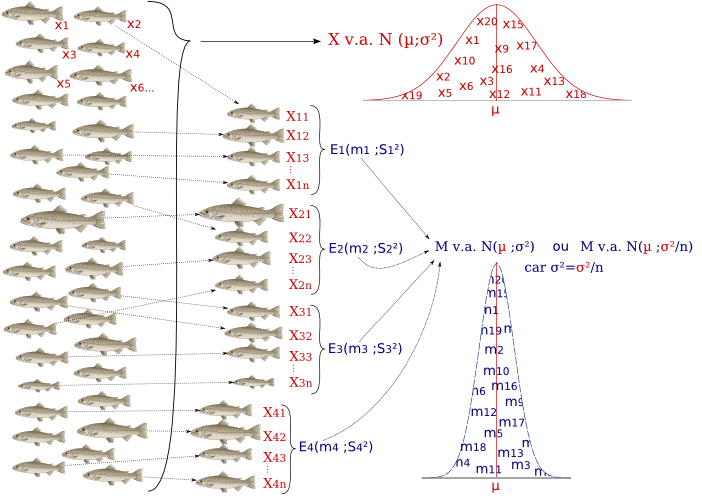
\includegraphics[width=1\linewidth]{illustrations/tcl}
	\caption{}
	\label{fig:tcl}
	\source{\url{http://webapps.fundp.ac.be/biostats/biostat/modules/module70/page4.html}, consultée le 28/09/2018.}
	
\end{figure}




\end{document}          

